\documentclass[UTF8,11pt,openany]{ctexbook}
\usepackage{titlesec}		%标题样式
\usepackage{geometry}		%页面间距
\usepackage{microtype}		%单词间距自动调整
\usepackage{graphicx}		%插入图片   
\usepackage{mathptmx}		%使用times字体
\usepackage{fancyhdr}		%页眉页脚,不用中文
\usepackage{clrscode3e}		%clrs package 
\usepackage{enumitem}
 

%行间距
\linespread{1}
%页眉
\pagestyle{fancy}
\renewcommand{\chaptermark}[1]{ \markboth{#1}{} }	%页面用英文, 小写
\renewcommand{\sectionmark}[1]{ \markright{#1}{} }

\renewcommand\headrulewidth{0pt}
\lhead{chapter \thechapter \ \leftmark}
\rhead{\thesection \ \rightmark}
%页面间距
\newgeometry{left = 3 cm, right=3 cm,top=1.5cm,bottom=1.5cm}
%文中一些字体
\newcommand{\bold}[1]{\textbf{#1}}
\newcommand{\bolditalic}[1]{\textbf{\textit{#1}}}
\newcommand{\point}[1]{\noindent{\textbf{#1}}}
  
\newenvironment{myitemize}
{ \begin{itemize}
	\setlength{\itemsep}{0pt}
	\setlength{\parskip}{0pt}
	\setlength{\parsep}{0pt}     }
{ \end{itemize}                  }

\newenvironment{myenumerate}
{ \begin{enumerate}
	\setlength{\itemsep}{0pt}
	\setlength{\parskip}{0pt}
	\setlength{\parsep}{0pt}     }
{ \end{enumerate}                  }


%重定义chapter, section的样式及行间距,不用cbook的默认样式
\titlespacing{\chapter}{0pt}{2.5ex plus 1ex minus .2ex}{1.3ex plus .2ex}
\titleformat{\chapter}{\huge\bfseries}{\thechapter}{2em}{}
\titleformat{\section}{\Large\bfseries}{\thesection}{1em}{}

 
\begin{document}


\chapter{Red Black Tree}
\section{definition}

A \bolditalic{red-black} tree is a binary search tree that satisfies the following \bolditalic{red-black} properties:

1. Every node is either red or black.

2. The root is black.

3. Every leaf (NIL) is black.

4. If a node is red, then both its children are black.

5. For each node, all simple paths from the node to descendant leaves contain the same number of black nodes.
 
 
注:
  The "usual" red-black trees can have two red children (but no red child to a red node) and correspond to 2-4 trees.
  
  
\begin{figure}[h] %figure环境,h默认参数是可以浮动,不是固定在当前位置。如果要不浮动,你就可以使用大写float宏包的H参数,固定图片在当前位置,禁止浮动。
	\centering %使图片居中显示
	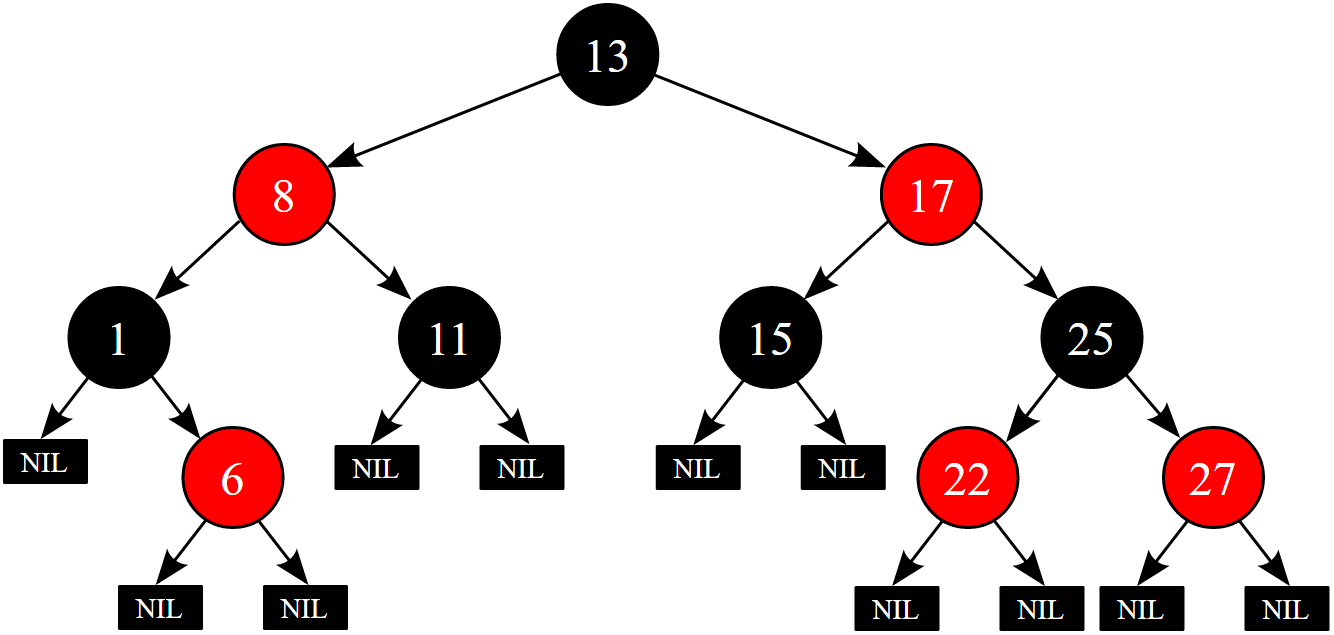
\includegraphics[width=0.6\textwidth]{rb_sample.png} %中括号中的参数是设置图片充满文档的大小,你也可以使用小数来缩小图片的尺寸。
	\caption{red black tree sample, node 25 has two red children.} %caption是用来给图片加上图题的
	\label{red_black_tree_sample1} %这是添加标签,方便在文章中引用图片。
\end{figure}%figure环境

 

\point{Proposition 13.1}\\
A red-black tree with n internal nodes has height at most 2lg(n+1).

\point{Proof} We start by showing that the subtree rooted at any node x contains at least
$2^{bh(x)} - 1$ internal nodes. We prove this claim by induction on the height of x.If
the height of x is 0, then x must be a leaf (T:nil), and the subtree rooted at x indeed
contains at least $2^{bh(x)} - 1 = 2^0 - 1 = 0$ internal nodes. For the inductive step,
consider a node x that has positive height and is an internal node with two children.
Each child has a black-height of either bh(x) or bh(x) - 1. , depending on whether
its color is red or black, respectively. Since the height of a child of x is less than
the height of x itself, we can apply the inductive hypothesis to conclude that each
child has at least $2^{bh(x)} - 1$ internal nodes. Thus, the subtree rooted at x contains
at least  $(2^{bh(x)-1} - 1) +2^{bh(x)-1} - 1) +1=2^{bh(x)} - 1 $ internal nodes, which proves
the claim.

\newpage 
\section{rotations}

\begin{figure}[h] %figure环境,h默认参数是可以浮动,不是固定在当前位置。如果要不浮动,你就可以使用大写float宏包的H参数,固定图片在当前位置,禁止浮动。
	\centering %使图片居中显示
	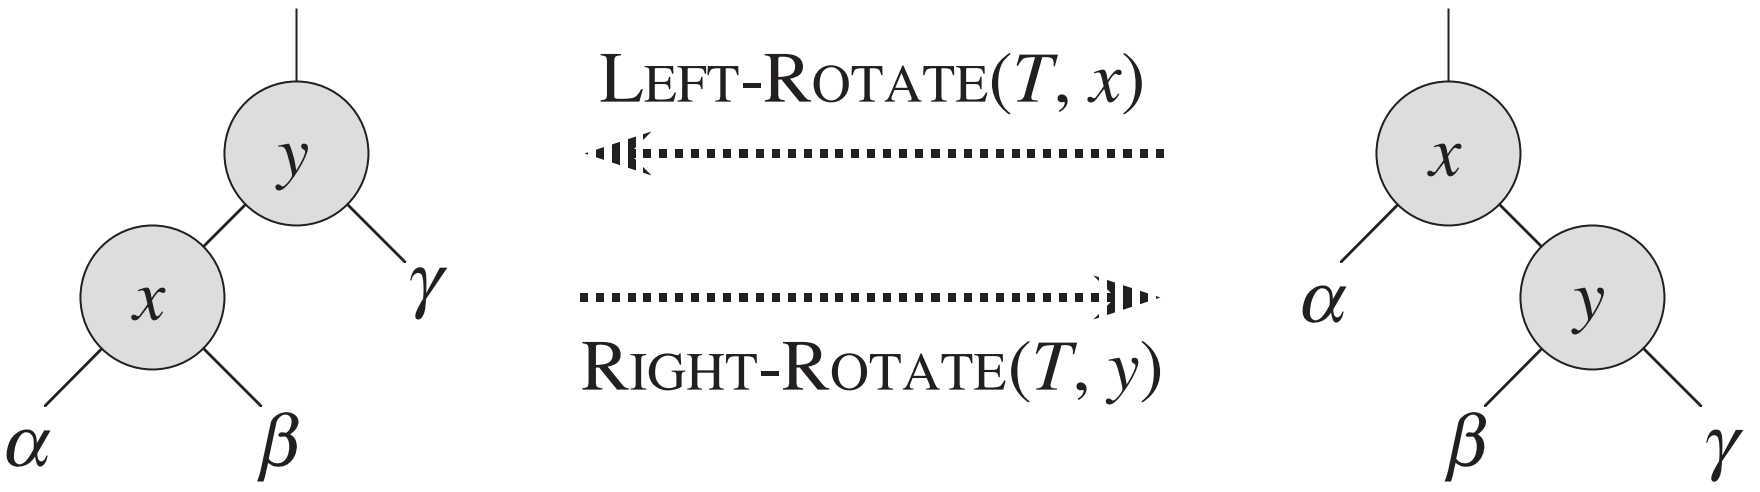
\includegraphics[width=0.6\textwidth]{rb-rotate.png} %中括号中的参数是设置图片充满文档的大小,你也可以使用小数来缩小图片的尺寸。
	\caption{The rotation operations on a binary search tree. The operation LEFT-ROTATE(T,x) transforms the configuration of the two nodes on the right into the configuration on the left by changing a constant number of pointers.
	} %caption是用来给图片加上图题的
	\label{red_black_tree_sample1} %这是添加标签,方便在文章中引用图片。
\end{figure}%figure环境
 
\begin{codebox}
	\Procname{$\proc{left-rotate}(T,x)$}
	\li    $ y \gets \attrib{x}{right} $
	\li    $ \attrib{x}{right} \gets \attrib{y}{left}  $ 
	\li    \If $\attrib{y}{left} \ne \attrib{T}{nil}$
	\li        \Then   $\attribb{y}{left}{p} \gets x$
		   \End
    \li    $ \attrib{y}{p} \gets \attrib{x}{p} $
	\li    \If  $\attrib{x}{p} \isequal \attrib{T}{nil}$
	\li        \Then    $\attrib{T}{root} \gets y$
	\li    \ElseIf   $ x \isequal \attribb{x}{p}{left}$
	\li        \Then $ \attribb{x}{p}{left} \gets y$
	\li    \Else  $ \attribb{x}{p}{right} \gets y$
	       \End
	\li    $\attrib{y}{left} \gets x$
	\li    $ \attrib{x}{p} \gets y $
\end{codebox}
 
\begin{codebox}
	\Procname{$\proc{right-rotate}(T,y)$}
	\li    $ x \gets \attrib{y}{left} $
	\li    $ \attrib{y}{left} \gets \attrib{x}{right}  $ 
	\li    \If $\attrib{x}{right} \ne \attrib{T}{nil}$
	\li        \Then   $\attribb{x}{right}{p} \gets y$
	       \End
	\li    $ \attrib{x}{p} \gets \attrib{y}{p} $
	\li    \If  $\attrib{y}{p} \isequal \attrib{T}{nil}$
	\li        \Then    $\attrib{T}{root} \gets x$
	\li    \ElseIf   $ y \isequal \attribb{y}{p}{left}$
	\li        \Then $ \attribb{y}{p}{left} \gets x$
	\li    \Else  $ \attribb{y}{p}{right} \gets x$
	\End
	\li    $\attrib{x}{right} \gets y$
	\li    $ \attrib{y}{p} \gets x $
\end{codebox}

\newpage 
\section{insertion}
\begin{codebox}
	\Procname{$\proc{rb-insert}(T,z)$}
	\li    $ y \gets \attrib{T}{nil} $
	\li    $ x \gets \attrib{T}{root} $
    \li     \While $ x \ne  \attrib{T}{nil}$ 
    \li     \Do $ y \gets x $
    \li         \If   $ \attrib{z}{key} < \attrib{x}{key} $
    \li         \Then $ x \gets \attrib{x}{left} $
    \li         \Else $ x \gets \attrib{x}{right} $
    			\End
            \End
    \li     $\attrib{z}{p} \gets y$ 
    \li         \If   $ y \isequal \attrib{T}{nil} $
    \li         \Then $  \attrib{T}{root}  \gets z $
    \li         \ElseIf $ \attrib{z}{key} < \attrib{y}{key}$
    \li         \Then   $ \attrib{y}{left}  \gets z  $
    \li  		\ElseNoIf  $ \attrib{y}{right}  \gets z  $    				
   				\End
   	\li    $ \attrib{z}{left}  \gets \attrib{T}{nil}$
   	\li    $ \attrib{z}{right}  \gets \attrib{T}{nil}$
   	\li    $ \attrib{z}{color}  \gets \const{red}$
	\li 			 $\proc{rb-insert-fixup}(T,z)$	
\end{codebox}

\begin{figure}[h] %figure环境,h默认参数是可以浮动,不是固定在当前位置。如果要不浮动,你就可以使用大写float宏包的H参数,固定图片在当前位置,禁止浮动。
	\centering %使图片居中显示
	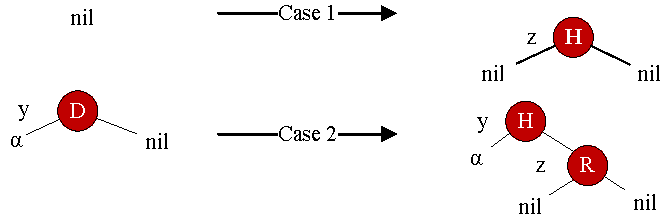
\includegraphics[width=0.8\textwidth]{vector/red-black-tree/insert/rb_insert_violated_cases.pdf} %中括号中的参数是设置图片充满文档的大小,你也可以使用小数来缩小图片的尺寸。
	\caption{rb insert violated cases that need to be fixed up } %caption是用来给图片加上图题的
	\label{rb_insert_violated_cases} %这是添加标签,方便在文章中引用图片。
\end{figure}%figure环境

\begin{codebox}
	\Procname{$\proc{rb-insert-fixup}(T,z)$}
	\li     \While $  \attribb{z}{p}{color} \isequal \const{red}$ 
	\li     \Do \If   $ \attrib{z}{p} \isequal \attribbb{z}{p}{p}{left} $ 
	\li         \Then $ y \gets \attribbb{z}{p}{p}{right}  $
	\li				\If   $ \attrib{y}{color} \isequal \const{red}  $ 
	\li             \Then $ \attribb{z}{p}{color} \gets \const{black}  $ \RComment case1
	\li                   $ \attrib{y}{color} \gets \const{black} $
	\li                   $ \attribbb{z}{p}{p}{color} \gets \const{red} $
	\li                   $ z \gets \attribb{z}{p}{p} $                  \RComment case1
	\li             \Else \If $z \isequal \attribb{z}{p}{right}$
	\li                   \Then $ z \gets \attrib{z}{p}  $				\RComment case2
	\li	                         $\proc{left-rotate}(T,z)$			    \RComment case2
						  \End
    \li                   $\attribb{z}{p}{color} \gets \const{black} $   \RComment case3
    \li                   $\attribbb{z}{p}{p}{color} \gets \const{red} $
 	\li	                  $\proc{right-rotate}(T,\attribb{z}{p}{p})$     \RComment case3
					\End   
	\li         \Else  (same as \kw{then} clause 	with “right” and “left” exchanged)
				\End
			\End
	\li     $\attribb{T}{root}{color} \gets \const{black} $	
\end{codebox}



\newpage 
\subsection{rb insert fixup cases explained}
\begin{figure}[h] %figure环境,h默认参数是可以浮动,不是固定在当前位置。如果要不浮动,你就可以使用大写float宏包的H参数,固定图片在当前位置,禁止浮动。
	\centering %使图片居中显示
	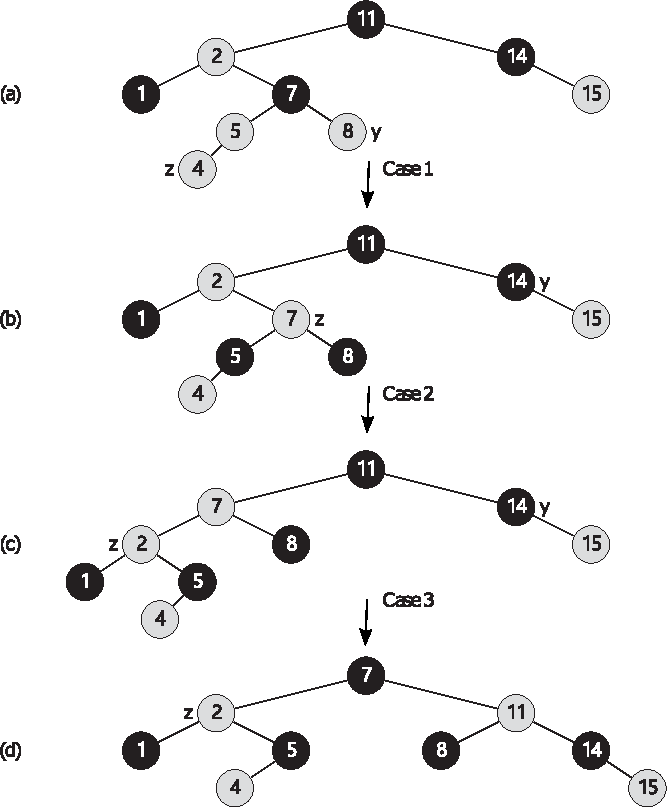
\includegraphics[width=0.8\textwidth]{vector/red-black-tree/insert/rb_insert_fix_cases.pdf} %中括号中的参数是设置图片充满文档的大小,你也可以使用小数来缩小图片的尺寸。
	\caption{\noindent{The} cases in $ \proc{rb-insert-fixup}  $.  } %caption是用来给图片加上图题的
	\label{rb_insert_fix_cases} %这是添加标签,方便在文章中引用图片。
\end{figure}%figure环境
\noindent(a) A node z after insertion. Because both z
and its parent z:p are red, a violation of property 4 occurs. Since z’s uncle y is red, case 1 in the
code applies. We recolor nodes and move the pointer z up the tree, resulting in the tree shown in (b).

\noindent Once again, z and its parent are both red, but z’s uncle y is black. Since z is the right child of z:p,
case 2 applies. We perform a left rotation, and the tree that results is shown in (c).

\noindent Now, z is the left
child of its parent, and case 3 applies. Recoloring and right rotation yield the tree in (d), which is a
legal red-black tree.

\subsection{Analysis}
What is the running time of RB-INSERT? Since the height of a red-black tree on n
nodes is O(lg n), lines 1–16 of RB-INSERT take O(lg n) time. In RB-INSERTFIXUP, the while loop repeats only if case 1 occurs, and then the pointer z moves
two levels up the tree. The total number of times the while loop can be executed
is therefore O(lg n). Thus, RB-INSERT takes a total of O(lg n) time. Moreover, it
never performs more than two rotations, since the while loop terminates if case 2
or case 3 is executed.

\newpage
\twocolumn 
\section{delete}
\begin{codebox}
\Procname{$\proc{rb-transplant}(T,u,v)$} 
\li    \If $\attrib{u}{p} \isequal \attrib{T}{nil}$
\li        \Then   $\attrib{T}{root} \gets v$
\li    \ElseIf    $u \isequal \attribb{u}{p}{left}$
\li        \Then    $\attribb{u}{p}{left} \gets v$
\li    \Else    $\attribb{u}{p}{right} \gets v$
       \End
\li    $\attrib{v}{p} \gets \attrib{u}{p}$
\end{codebox}

\
\newline
\newline
\newline
\newline
\newline
\newline
\newline
\newline
\newline
\newline
\newline
\newline
\newline
\newline
\

\begin{codebox}
	\Procname{$\proc{rb-delete-fixup}(T,x)$} 
	\li  \While $ x \ne  \attrib{T}{root}$ and  $\attrib{x}{color} \isequal \const{black}$
	\li  \Do  \If $x \isequal \attribb{x}{p}{left}$
	\li   	\Then 
	$ w \gets \attribb{x}{p}{right} $
	\li		   \If $ \attrib{w}{color} \isequal \const{red}$
	\li		     \Then 
	$ \attrib{w}{color} \gets \const{black} $    				\RComment case1
	\li			 $ \attribb{x}{p}{color} \gets \const{red} $
	\li  			 $ \proc{left-rotate}(T,\attrib{x}{p}) $
	\li			 $ w \gets \attribb{x}{p}{right} $      		\RComment case1
	\End
	\li          \If $ \attribb{w}{left}{color} \isequal \const{black}$ and $ \attribb{w}{right}{color} \isequal \const{black} $ 	
	\li            \Then 
	$ \attrib{w}{color} \gets \const{red} $    					\RComment case2	  
	\li            $ x \gets \attrib{x}{p} $     				\RComment case2
	\li          \Else
	\If $ \attribb{w}{right}{color} \isequal \const{black} $	
	\li              \Then 
	$ \attribb{w}{left}{color} \gets \const{black} $            \RComment case3
	\li 			   $ \attrib{w}{color} \gets \const{red}   $	
	\li 			   $\proc{right-rotate}(\attrib{T}{w})$	
	\li 			   $w \gets \attribb{x}{p}{right}$          \RComment case3	 
	\End
	\li            $ \attrib{w}{color} \gets \attribb{x}{p}{color} $  \RComment case4
	\li            $ \attribb{x}{p}{color} \gets \const{black} $
	\li            $ \attribb{w}{right}{color} \gets \const{black} $
	\li 			 $\proc{left-rotate}(T,\attrib{x}{p})$	
	\li            $ x \gets \attrib{T}{root} $                      \RComment case4
	             \End
	\li        \Else (same as \kw{then} clause with "right" and "left" exchanged)
	           \End
	      \End
	\li  $ \attrib{x}{color} \gets \const{black} $
\end{codebox}

\newpage 
\


\begin{codebox}
	\Procname{$\proc{rb-delete}(T,z)$} 
	\li    $y \gets z$
	\li    $\id{y-original-color} \gets \attrib{y}{color}$
	
	\li    \If $ \attrib{z}{left} \isequal \attrib{T}{nil} $
	\li        \Then  $ x  \gets \attrib{z}{right}$
	\li               $ \proc{rb-transplant}(T,z,\attrib{z}{right}) $
	\li    \ElseIf    $\attrib{z}{right} \isequal \attrib{T}{nil} $
	\li        \Then  $ x  \gets \attrib{z}{left} $
	\li               $ \proc{rb-transplant}(T,z,\attrib{z}{left}) $
	\li    \Else  $ y \gets \proc{tree-minimum}(\attrib{z}{right}) $
	\li           $ \id{y-original-color} \gets \attrib{y}{color} $  			  
	\li           $ x \gets \attrib{y}{right} $       
	\li           \If $ \attrib{y}{p} \isequal  z $		
	\li             \Then $ \attrib{x}{p}\gets y $
	\li           \Else  $ \proc{rb-transplant}(T,y,\attrib{y}{right}) $ 
	\li                  $ \attrib{y}{right} \gets \attrib{z}{right} $
	\li                  $ \attribb{y}{right}{p} \gets y $ 
	\End
	\li           $ \proc{rb-transplant}(T,z,y) $ 
	\li           $ \attrib{y}{left} \gets \attrib{z}{left} $ 
	\li           $ \attribb{y}{left}{p} \gets y $ 
	\li           $ \attrib{y}{color} \gets \attrib{z}{color} $ 
	\End
	
	\li    \If $ \id{y-original-color} \isequal \const{black} $
	\li       \Then $\proc{rb-delete-fixup}(\attrib{T}{x})$
	\End
\end{codebox}

\newpage
\onecolumn

\begin{codebox}
	\Procname{$\proc{rb-delete}(T,z)$} 
	\li    $y \gets z$
	\li    $\id{y-original-color} \gets \attrib{y}{color}$
	
	\li    \If $ \attrib{z}{left} \isequal \attrib{T}{nil} $
	\li        \Then  $ x  \gets \attrib{z}{right}$
	\li               $ \proc{rb-transplant}(T,z,\attrib{z}{right}) $
	\li    \ElseIf    $\attrib{z}{right} \isequal \attrib{T}{nil} $
	\li        \Then  $ x  \gets \attrib{z}{left} $
	\li               $ \proc{rb-transplant}(T,z,\attrib{z}{left}) $
	\li    \Else  $ y \gets \proc{tree-minimum}(\attrib{z}{right}) $
	\li           $ \id{y-original-color} \gets \attrib{y}{color} $  			  
	\li           $ x \gets \attrib{y}{right} $       
	\li           \If $ \attrib{y}{p} \isequal  z $		
	\li             \Then $ \attrib{x}{p}\gets y $
	\li           \Else  $ \proc{rb-transplant}(T,y,\attrib{y}{right}) $ 
	\li                  $ \attrib{y}{right} \gets \attrib{z}{right} $
	\li                  $ \attribb{y}{right}{p} \gets y $ 
	\End
	\li           $ \proc{rb-transplant}(T,z,y) $ 
	\li           $ \attrib{y}{left} \gets \attrib{z}{left} $ 
	\li           $ \attribb{y}{left}{p} \gets y $ 
	\li           $ \attrib{y}{color} \gets \attrib{z}{color} $ 
	\End
	
	\li    \If $ \id{y-original-color} \isequal \const{black} $
	\li       \Then $\proc{rb-delete-fixup}(\attrib{T}{x})$
	\End
\end{codebox}

\begin{figure}[h] %figure环境,h默认参数是可以浮动,不是固定在当前位置。如果要不浮动,你就可以使用大写float宏包的H参数,固定图片在当前位置,禁止浮动。
	\centering %使图片居中显示
	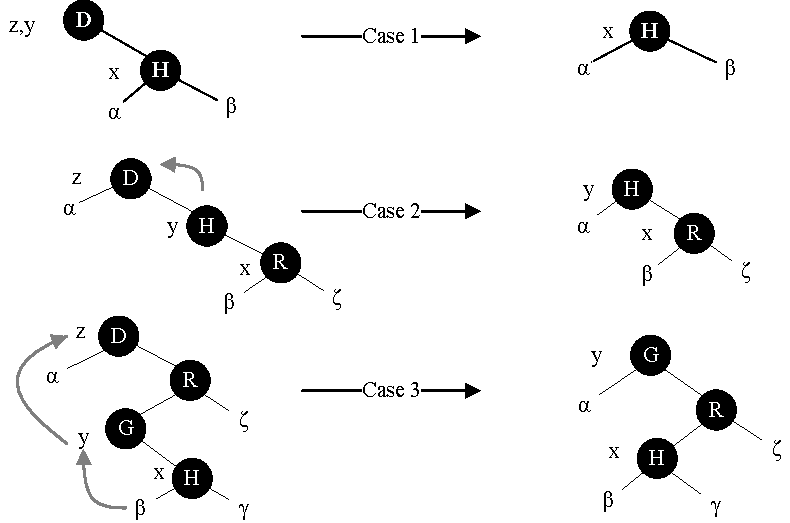
\includegraphics[width=1\textwidth]{vector/red-black-tree/delete/delete_cases.pdf} %中括号中的参数是设置图片充满文档的大小,你也可以使用小数来缩小图片的尺寸。
	\caption{\noindent{The} cases in $ \proc{rb-delete}  $.  } %caption是用来给图片加上图题的
	\label{red_black_delete_cases} %这是添加标签,方便在文章中引用图片。
\end{figure}%figure环境

\newpage

\begin{figure}[h] %figure环境,h默认参数是可以浮动,不是固定在当前位置。如果要不浮动,你就可以使用大写float宏包的H参数,固定图片在当前位置,禁止浮动。
	\centering %使图片居中显示
	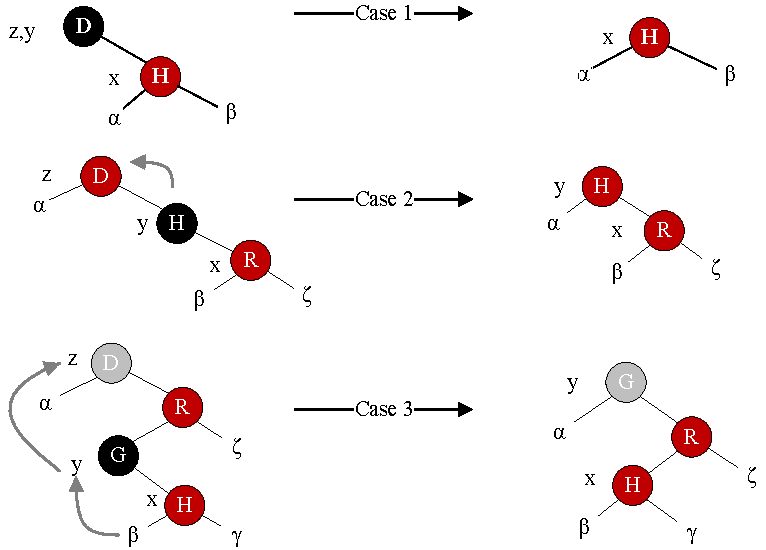
\includegraphics[width=1\textwidth]{vector/red-black-tree/delete/delete_cases2.pdf} %中括号中的参数是设置图片充满文档的大小,你也可以使用小数来缩小图片的尺寸。
	\caption{if y-original-color is black, the cases we need to fixup} %caption是用来给图片加上图题的
	\label{red_black_delete_cases} %这是添加标签,方便在文章中引用图片。
\end{figure}%figure环境

\subsection{If y-original-color is black, we need to fix up.} 
\point{case1}
\begin{myenumerate}
	\item If Z is root, x is red, property 1 violated
	\item 2 if Z is not root, property 5 violated
\end{myenumerate}  
 
\point{case2}
\begin{myenumerate}
	\item If  x is red and z is red, property 4 violated
	\item black height of the subtree rooted at z minus 1, property 5 violated.
\end{myenumerate}  
 
\point{case3}
\begin{myenumerate}
	\item If  x is red and node R is red, property 4 violated 
	\item black height of the subtree rooted at z minus 1, property 5 violated.
\end{myenumerate}  

\point{PS. red black tree properties:}\\
1. Every node is either red or black.\\
2. The root is black.\\
3. Every leaf (NIL) is black.\\
4. If a node is red, then both its children are black.\\
5. For each node, all simple paths from the node to descendant leaves contain the same number of black nodes.

\newpage
\subsection{fix up cases when delete}
\begin{figure}[h] %figure环境,h默认参数是可以浮动,不是固定在当前位置。如果要不浮动,你就可以使用大写float宏包的H参数,固定图片在当前位置,禁止浮动。
	\centering %使图片居中显示
	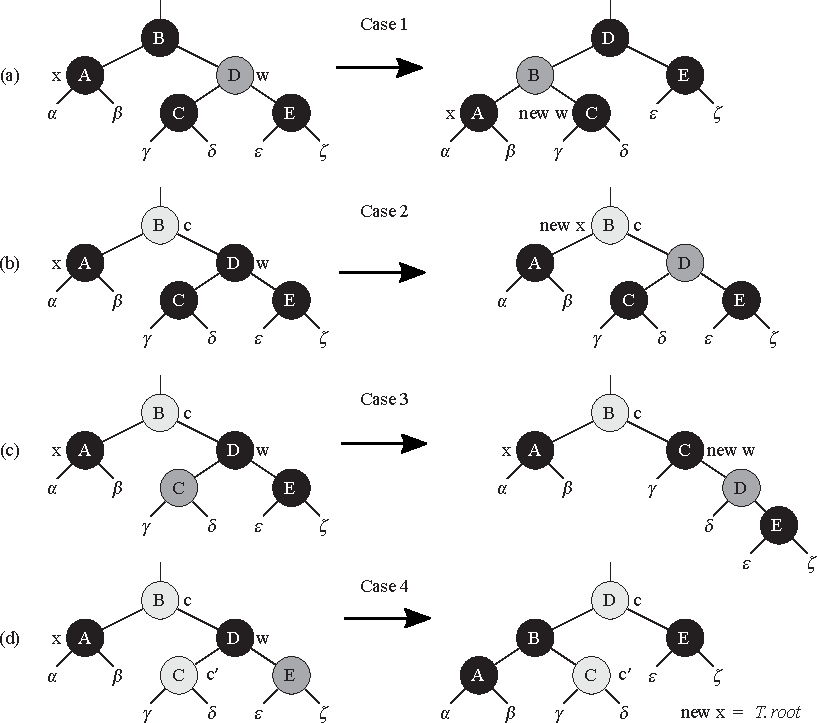
\includegraphics[width=1\textwidth]{vector/red-black-tree/delete/fixup-cases.pdf} %中括号中的参数是设置图片充满文档的大小,你也可以使用小数来缩小图片的尺寸。
	\caption{\noindent{The} cases in the while loop of the procedure $ \proc{RB-DELETE-FIXUP}  $.  } %caption是用来给图片加上图题的
	\label{red_black_tree_sample1} %这是添加标签,方便在文章中引用图片。
\end{figure}%figure环境

\begin{myitemize}
	\item {Darkened} nodes have color attributes \const{black}, 
	\item heavily shaded nodes have color attributes \const{red}, 
	\item and lightly shaded nodes have color attributes represented by c and $c'$, which may be either \const{red} or \const{black}. 
\end{myitemize}  
The letters
$\alpha,\beta...\zeta$ represent arbitrary subtrees. Each case transforms the configuration on the left into the
configuration on the right by changing some colors and/or performing a rotation. Any node pointed
to by x has an extra black and is either doubly black or red-and-black. Only case 2 causes the loop to
repeat.

\newpage 
\subsection{Detailed explanation for the cases in the while loop of the procedure \proc{RB-DELETE-FIXUP}   . }

\point{Case 1: x's sibling w is red }\\
Case 1 (lines 5–8 of RB-DELETE-FIXUP and Figure 13.7(a)) occurs when node w,
the sibling of node x, is red. Since w must have black children, we can switch the
colors of w and $\attrib{x}{p}$ and then perform a left-rotation on $\attrib{x}{p}$ without violating any
of the red-black properties. The new sibling of x, which is one of w's children
prior to the rotation, is now black, and thus we have converted case 1 into case 2,
3, or 4.
Cases 2, 3, and 4 occur when node w is black; they are distinguished by the
colors of w's children.
\\

\point{Case 2: x's sibling w is black, and both of w's children are black}\\
In case 2 (lines 10–11 of RB-DELETE-FIXUP and Figure 13.7(b)), both of w's
children are black. Since w is also black, we take one black off both x and w,
leaving x with only one black and leaving w red. To compensate for removing
one black from x and w, we would like to add an extra black to $\attrib{x}{p}$, which was
originally either red or black. We do so by repeating the \kw{while} loop with $\attrib{x}{p}$ as
the new node x. Observe that if we enter case 2 through case 1, the new node x
is red-and-black, since the original $\attrib{x}{p}$ was red. Hence, the value c of the color
attribute of the new node x is RED, and the loop terminates when it tests the loop
condition. We then color the new node x (singly) black in line 23.
\\

\point{Case 3: x's sibling w is black, w's left child is red, and w's right child is black}\\
Case 3 (lines 13–16 and Figure 13.7(c)) occurs when w is black, its left child
is red, and its right child is black. We can switch the colors of w and its left
child $\attrib{w}{left}$ and then perform a right rotation on w without violating any of the
red-black properties. The new sibling w of x is now a black node with a red right
child, and thus we have transformed case 3 into case 4.
\\

\point{Case 4: x's sibling w is black, and w's right child is red}\\
Case 4 (lines 17–21 and Figure 13.7(d)) occurs when node x's sibling w is black
and w's right child is red. By making some color changes and performing a left rotation on $\attrib{x}{p}$, we can remove the extra black on x, making it singly black, without
violating any of the red-black properties. Setting x to be the root causes the \kw{while}
loop to terminate when it tests the loop condition.

\subsection{Analysis}
What is the running time of RB-DELETE? Since the height of a red-black tree of n
nodes is O(lg n), the total cost of the procedure without the call to RB-DELETEFIXUP takes O(lg n) time. Within RB-DELETE-FIXUP, each of cases 1, 3, and 4
lead to termination after performing a constant number of color changes and at
most three rotations. Case 2 is the only case in which the while loop can be repeated, and then the pointer x moves up the tree at most O(lg n) times, performing
no rotations. Thus, the procedure RB-DELETE-FIXUP takes O(lg n) time and performs at most three rotations, and the overall time for RB-DELETE is therefore
also O(lg n)



 
\chapter{reb black tree understanding}
\section{questions about deletion}
\subsubsection{the choose of y and x}
in rb-delete, choose which node as y and x in different cases?
\vspace{-10pt}

\begin{figure}[ht]
	\begin{minipage}[b]{0.45\linewidth}
	\centering
	  \begin{codebox}
	    \Procname{$\proc{rb-delete}(T,z)$} 
	    \li    $y \gets z$
	    \li    $\id{y-original-color} \gets \attrib{y}{color}$
	    
	    \li    \If $ \attrib{z}{left} \isequal \attrib{T}{nil} $
	    \li        \Then  $ x  \gets \attrib{z}{right}$
	    \li               $ \proc{rb-transplant}(T,z,\attrib{z}{right}) $
	    \li    \ElseIf    $\attrib{z}{right} \isequal \attrib{T}{nil} $
	    \li        \Then  $ x  \gets \attrib{z}{left} $
	    \li               $ \proc{rb-transplant}(T,z,\attrib{z}{left}) $
	    \li    \Else  $ y \gets \proc{tree-minimum}(\attrib{z}{right}) $
	    \li           $ \id{y-original-color} \gets \attrib{y}{color} $  			  
	    \li           $ x \gets \attrib{y}{right} $       
	    \li           \If $ \attrib{y}{p} \isequal  z $		
	    \li             \Then $ \attrib{x}{p}\gets y $
	    \li           \Else  $ \proc{rb-transplant}(T,y,\attrib{y}{right}) $ 
	    \li                  $ \attrib{y}{right} \gets \attrib{z}{right} $
	    \li                  $ \attribb{y}{right}{p} \gets y $ 
	    \End
	    \li           $ \proc{rb-transplant}(T,z,y) $ 
	    \li           $ \attrib{y}{left} \gets \attrib{z}{left} $ 
	    \li           $ \attribb{y}{left}{p} \gets y $ 
	    \li           $ \attrib{y}{color} \gets \attrib{z}{color} $ 
	    \End
	    
	    \li    \If $ \id{y-original-color} \isequal \const{black} $
	    \li       \Then $\proc{rb-delete-fixup}(\attrib{T}{x})$
	    \End
      \end{codebox}
	\label{fig:figure1}
	\end{minipage}
	\hspace{1cm}
	\begin{minipage}[b]{0.45\linewidth}
	\centering
	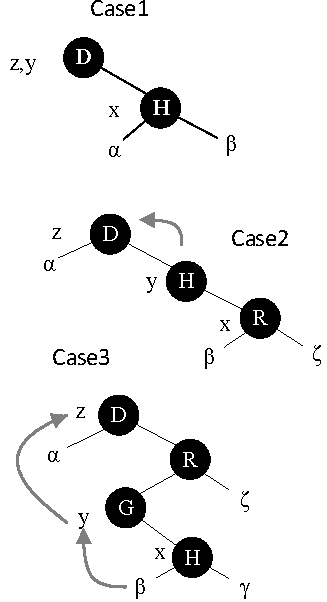
\includegraphics[width=0.8\textwidth]{vector/red-black-tree/delete/rb_delete_cases_single.pdf}
	\caption{3 cases in rb-delete}
	\label{fig:figure2}
	\end{minipage}
	\end{figure} 
	\vspace{-10pt}

	\begin{myitemize}
	\item z: the deleting node.
	\item 删除的3种case, 在case 1, 2, z 的node被抹去,z原来所在的node color也被抹去。
	\item case3 中,y节点替换z节点原来的位置,但y.color = z.color, 即z原来占位的节点,color没有丢失。
	但y原来所占的节点,color丢失了。
	\end{myitemize}  
	\point{综上,y用来表示丢失color的节点,x表示y的右孩子}






 

\end{document}